\chapter{Results}
\label{chap:results}

% intro results. relate to method.

\section{Comparsion with lightning data}

\begin{figure}[h]
    \centering
    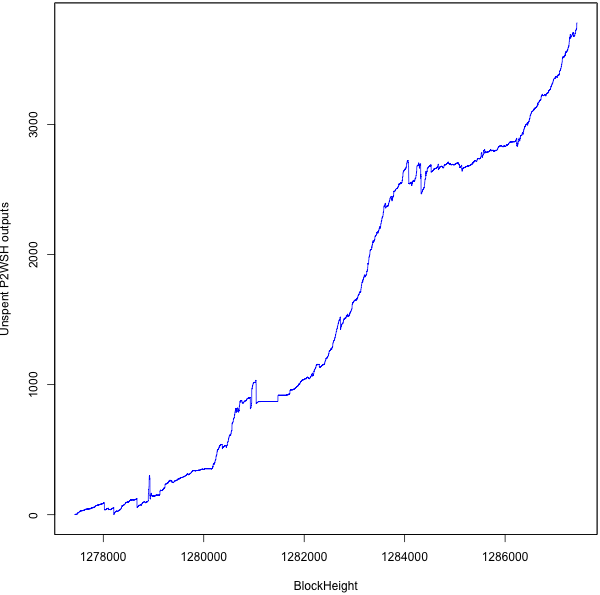
\includegraphics[width=10cm]{figures/bclnsizeTS.png}
    \caption{Maximum size of the ln based on unspent P2WSH outputs on the blockchain}
    \label{fig:htlc_bc}
\end{figure}

\begin{figure}[t]
    \centering
    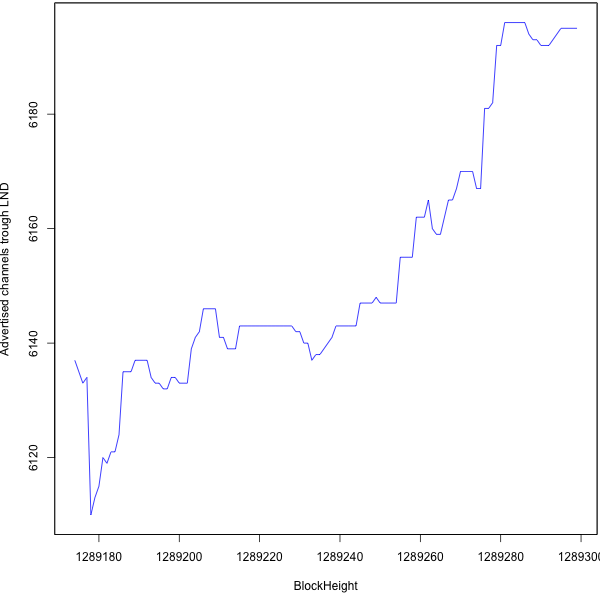
\includegraphics[width=10cm]{figures/lnsizeTS.png}
    \caption{Channel count from LN on testnet}
    \label{fig:htlc_bc}
\end{figure}

\section{Full runs}

\section{Other metrics}

\section{Clustering}

\begin{figure}[h]
    \centering
    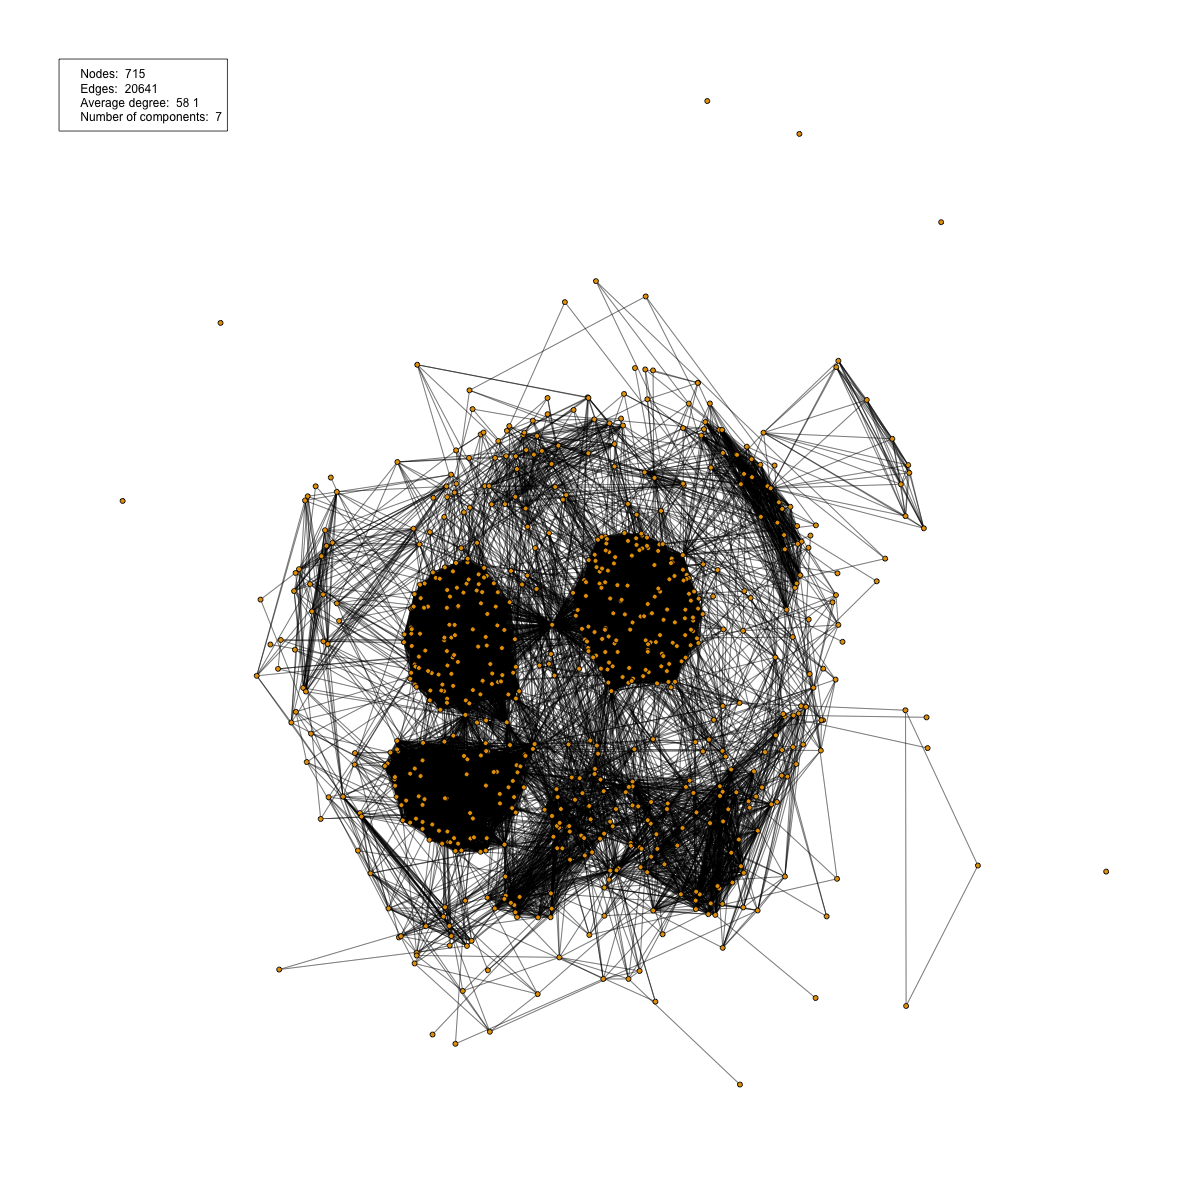
\includegraphics[width=14cm]{figures/graphs/cg_ln_mainnet_run1.png}
    \caption{Linked channels from LN mainnet run1}
    \label{fig:channelGraphLNTS}
\end{figure}

\begin{figure}[h]
    \centering
    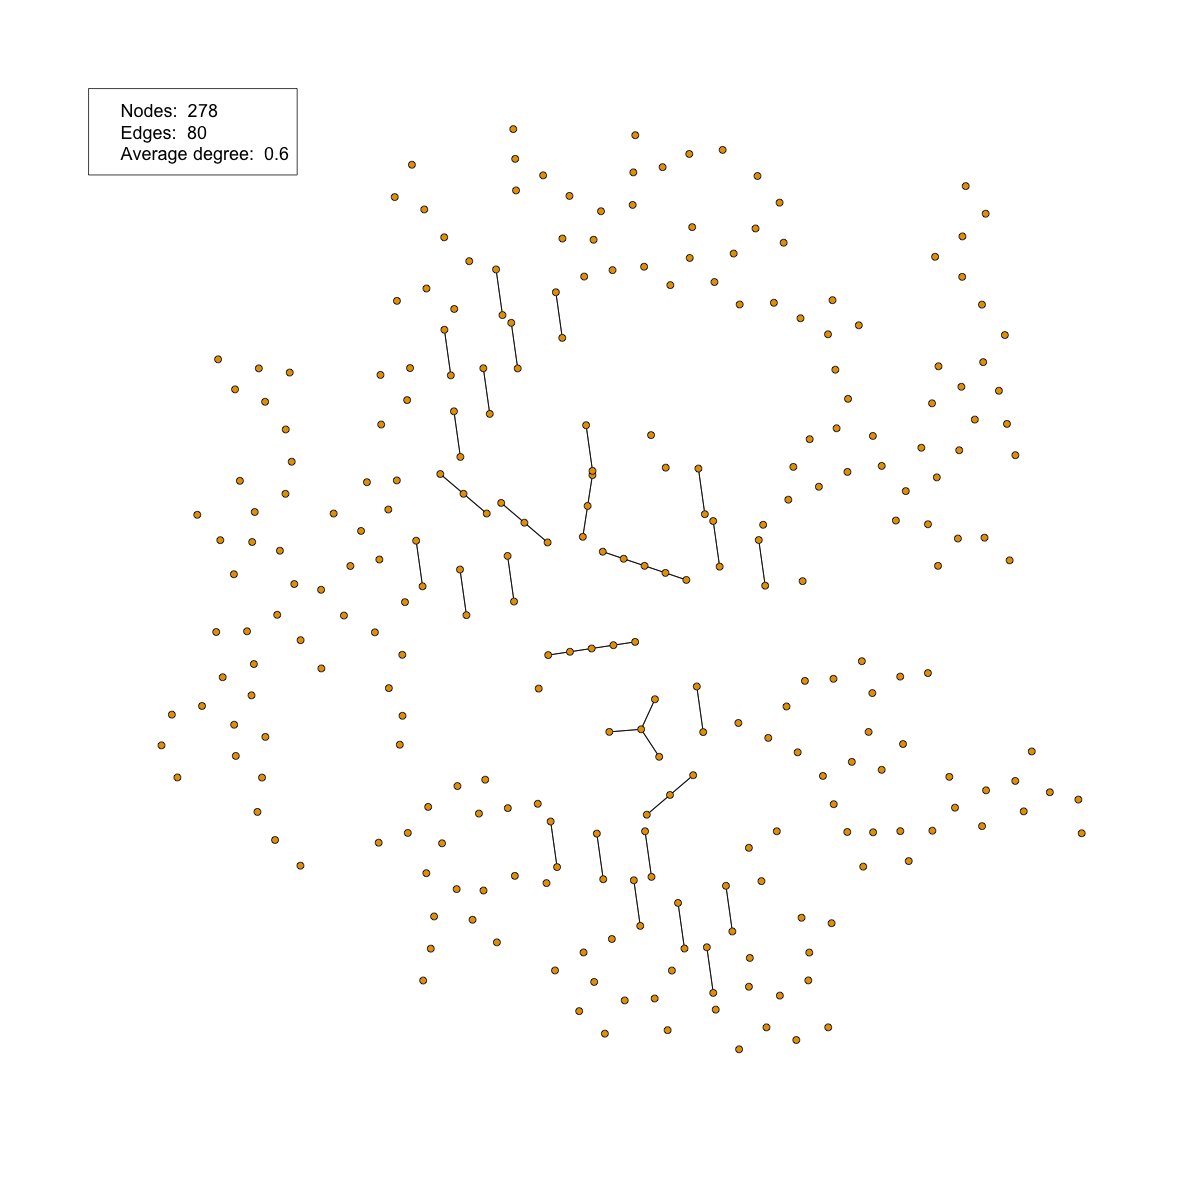
\includegraphics[width=14cm]{figures/graphs/cg_bc_mainnet_run1.png}
    \caption{Linked channels from BC mainnet run1}
    \label{fig:channelGraphLNTS}
\end{figure}